\part{Shaders}
\frame{\partpage}

\begin{frame}{Recap: processing pixels}
	\begin{columns}
		\begin{column}{0.5\textwidth}
			\begin{center}
				\pause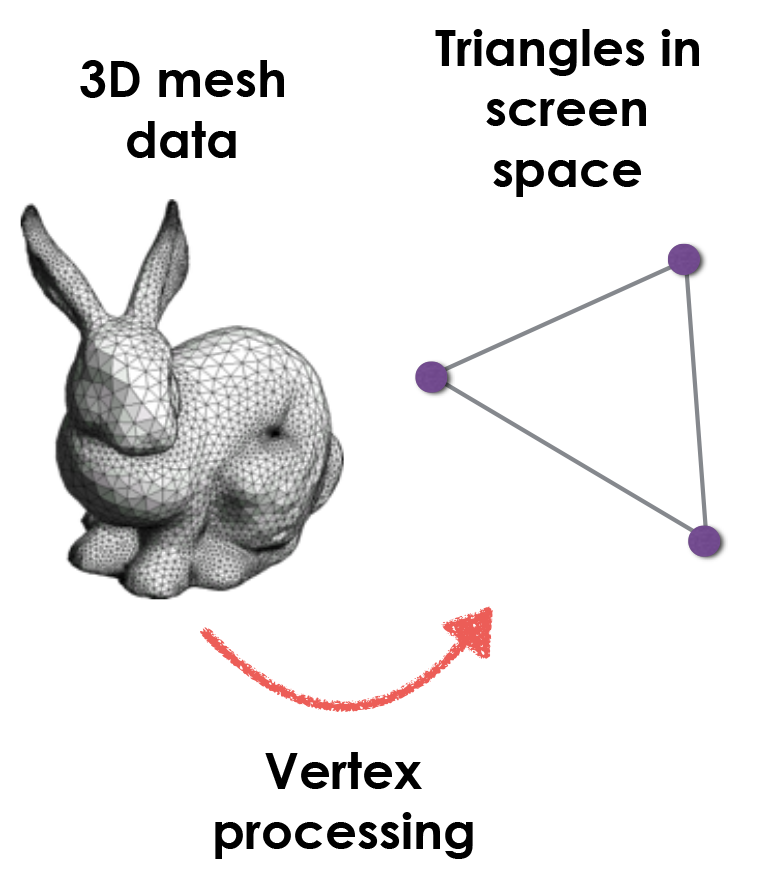
\includegraphics[height=0.85\textwidth]{vertex_processing}\\
			\end{center}
			Vertex processor \textbf{transforms} vertices and \textbf{projects} them into 2D screen space.
		\end{column}
		\begin{column}{0.5\textwidth}
			\begin{center}
				\pause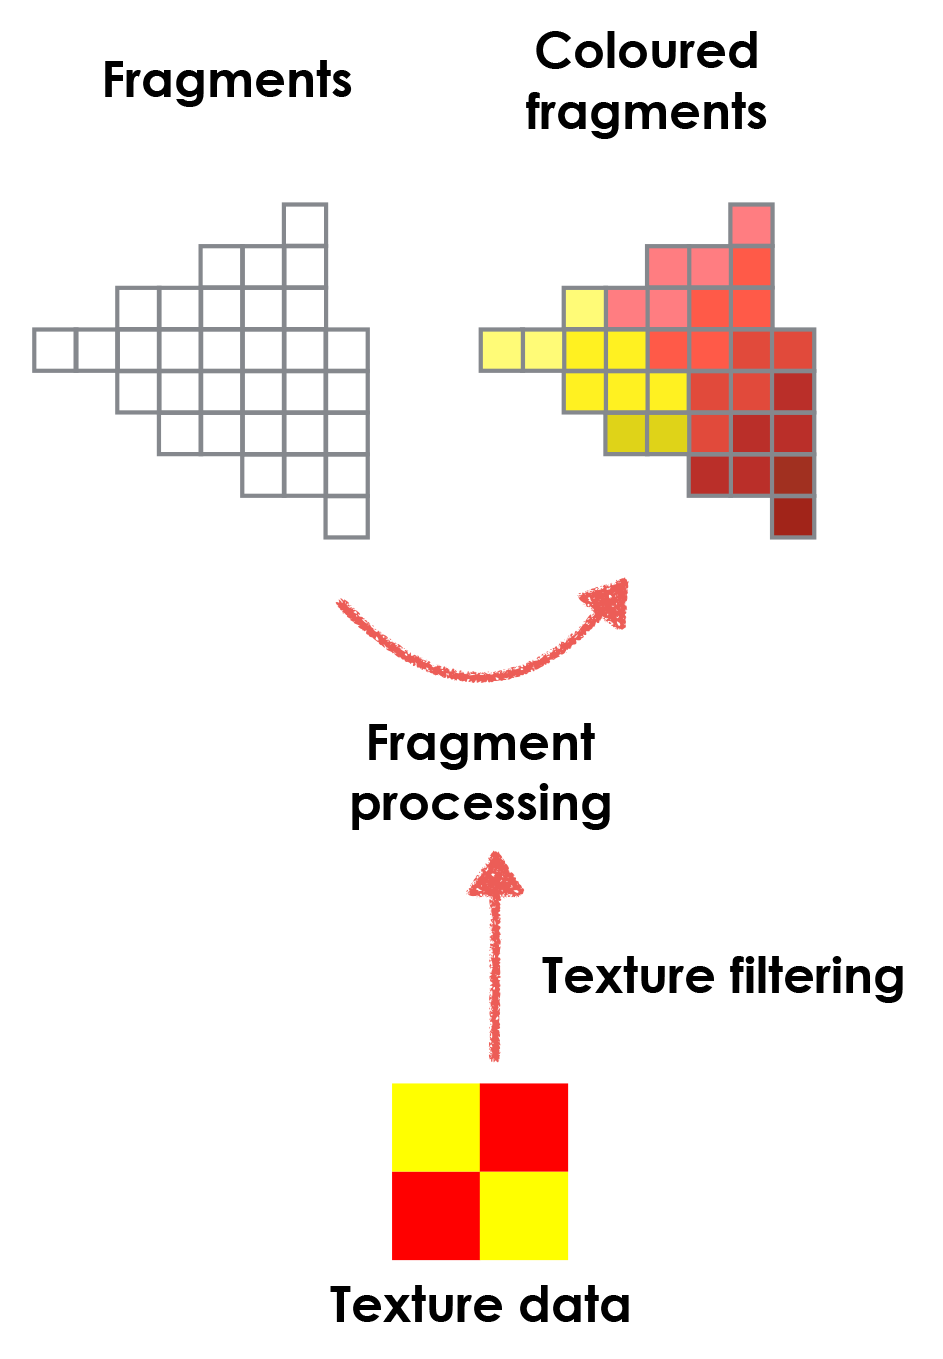
\includegraphics[height=0.85\textwidth]{fragment_processing}\\
			\end{center}
			Fragment processor determines the \textbf{colour} of each fragment covered by the triangle.
		\end{column}
	\end{columns}
\end{frame}

\begin{frame}{Vertex and fragment shaders}
	\begin{itemize}
		\pause\item The vertex processor and fragment processor are \textbf{programmable}
		\pause\item Programs for these units are called \textbf{shaders}
		\pause\item \textbf{Vertex shader}: responsible for geometric transformations, deformations, and projection
		\pause\item \textbf{Fragment shader}: responsible for the visual appearance of the surface
		\pause\item Vertex shader and fragment shader are separate programs,
			but the vertex shader can pass arbitrary values through to the fragment shader
	\end{itemize}
\end{frame}

\begin{frame}{Interpolation}
	\begin{columns}
		\begin{column}{0.5\textwidth}
			\begin{itemize}
				\pause\item The vertex shader sets a value for each vertex
				\pause\item So what is the value in the middle of the triangle?
				\pause\item The GPU \textbf{interpolates} the value across the triangle
			\end{itemize}
		\end{column}
		\begin{column}{0.45\textwidth}
			\pause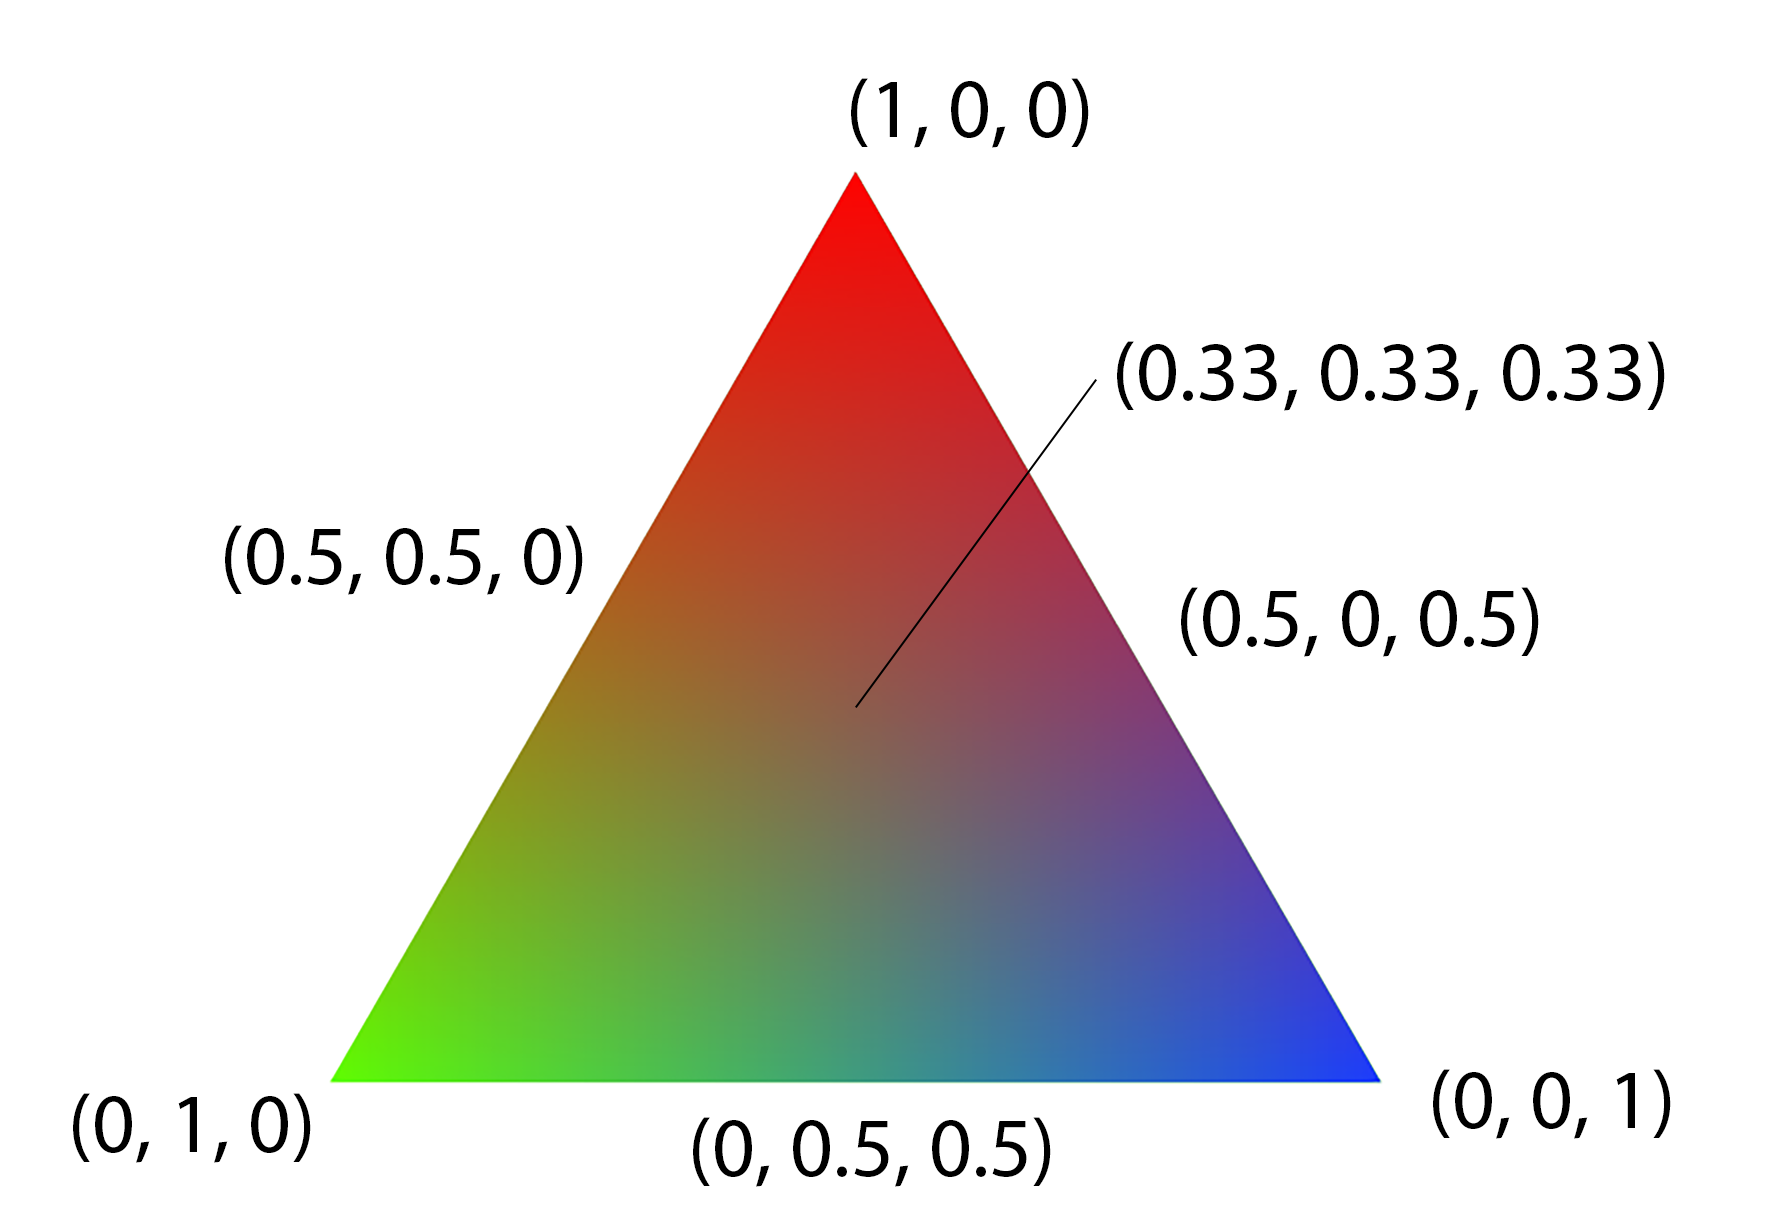
\includegraphics[width=\textwidth]{interpolation}
		\end{column}
	\end{columns}
\end{frame}